\documentclass[dvipdfmx,autodetect-engine, 12pt]{jsarticle}

\usepackage{ulem} % 取消線を引くためのパッケージ
\usepackage[dvipdfmx]{graphicx} % 画像を挿入するためのパッケージ
\usepackage{array} % 表の幅指定や自動改行に必要
\usepackage{enumitem}

% --- 参考文献用の設定 ---
\usepackage[backend=biber, style=numeric]{biblatex} % biblatexパッケージの使用
\addbibresource{report4.bib} % 先ほど作った別ファイルを指定（拡張子まで書く）
\usepackage{url} % WebサイトのURLを綺麗に出力するため

% --- section の文字サイズを小さくする設定 ---
\makeatletter
\renewcommand{\section}{%
  \@startsection{section}{1}{\z@}%
  {1.5ex \@plus .5ex \@minus .2ex}% 前の行との隙間
  {0.5ex \@plus .3ex}% 下の行との隙間
  {\normalfont\normalsize}% ← ここでサイズを \Large（少し大きめ）に指定
}
\makeatother

\begin{document}

% 課題のタイトル
\begin{center}

{\LARGE \bfseries 課題④\, ポートスキャンのパケット解析\par}

\end{center}

\vspace{1cm}

{\LARGE \uline{目的}} \\

\hangindent=1.5zw
\hangafter=0
\noindent
探査段階の中心となるポートスキャンの実習を行う．Nmap で探査中のパケットを調査する．パケットを分析することにより，探査の仕組みを確認する．

\vspace{1cm}

{\LARGE \uline{事前準備}} 

\begin{enumerate}
    \item server と router の VM を起動する．
    \item TCP の 3way handshake を調査する．
    \item ホスト検出，ポートスキャン手法について調査する．
    \item telnet と SSH の違いについて調査する．
\end{enumerate}

\vspace{1cm}

{\LARGE \uline{注意事項}}

\begin{enumerate}[label=・]
    \item 不用意にインターネット上のサーバに対して Nmap を利用してポートスキャンを行うと，スキャンを受けている側からすればアタックを受けているように見える．演習で構築した VM 以外のサーバ等に対してスキャンしないようにすること．
    \item 自分で構築，設定していない IP アドレスのマシンへの通信が勝手に発生している場合は，解析に含めなくてよい．
\end{enumerate}

\vspace{1cm}

{\LARGE \uline{手順}} 

\begin{enumerate}[label=(\arabic*)]
    \item Nmap を使ったホスト検出 \\
    サブゴール：探査用マシン(server)が属するネットワーク内で動作しているすべてのマシンをリストアップする．
    \noindent
    \begin{enumerate}[label=\arabic*, leftmargin=*]
        
        \item server で Wireshark を起動する．
        
        \item 次のコマンドを実行して IP アドレスの指定範囲をスキャンすることで動作しているマシンを探し，IP アドレスを確認する．（Wireshark でパケットを記録すること） \\
        \texttt{\# nmap -sn スキャン対象の IP アドレスの範囲} \\
        （例えば \texttt{nmap -sn 172.20.1.1-254} あるいは \texttt{nmap -sn 172.20.1.0/24} アドレスの範囲はあくまで例です．どの範囲を指定すべきかは各自で考えること．）解析に時間がかかる場合には，範囲を限定すること． \\
        ※ ネットワーク内のすべてのマシンが検出されていることを確認すること． \\
        \mbox{}[解説]：個々のパケットではなく TCP ストリームを解析したい場合には，解析したい TCP ストリーム中のパケットを選択し，右クリックして表示される Follow TCP Stream を選択する．表示されるウィンドウ中の文字色の違いを把握しておくこと．

        \vspace{\baselineskip}
        \quad
        コマンドの実行結果を図\ref{fig:ping_scan_terminal}に示す.

        \begin{figure}[htbp]
            \centering
            
\includegraphics[width=0.8\textwidth]{imgs/1/nmap_ping_scan_result_terminal.png} 
            \caption{pingスキャンの結果}
            \label{fig:ping_scan_terminal}
        \end{figure}

        \item パケット解析した結果（パケットをキャプチャした結果など）を用いて，OSI 参照モデルのどの層で，どのような手順で，どのように，どのような情報が，やり取りされてホスト検出の仕組みが，実現されているかをレポートで報告しなさい．
        
        \quad
        pingスキャンを実行した際にwiresharkでキャプチャされたパケットの一覧と各パケットの詳細について図
        \ref{fig:nmap_ping_scan_result_arp_request}, \ref{fig:nmap_ping_scan_result_arp_reply}, \ref{fig:nmap_ping_scan_result_dns}, \ref{fig:nmap_ping_scan_result_icmp}に示す.

        \\
        \quad

        図\ref{fig:nmap_ping_scan_result_arp_request}はARP応答パケットである.
        

        \begin{figure}[htbp]
            \centering
            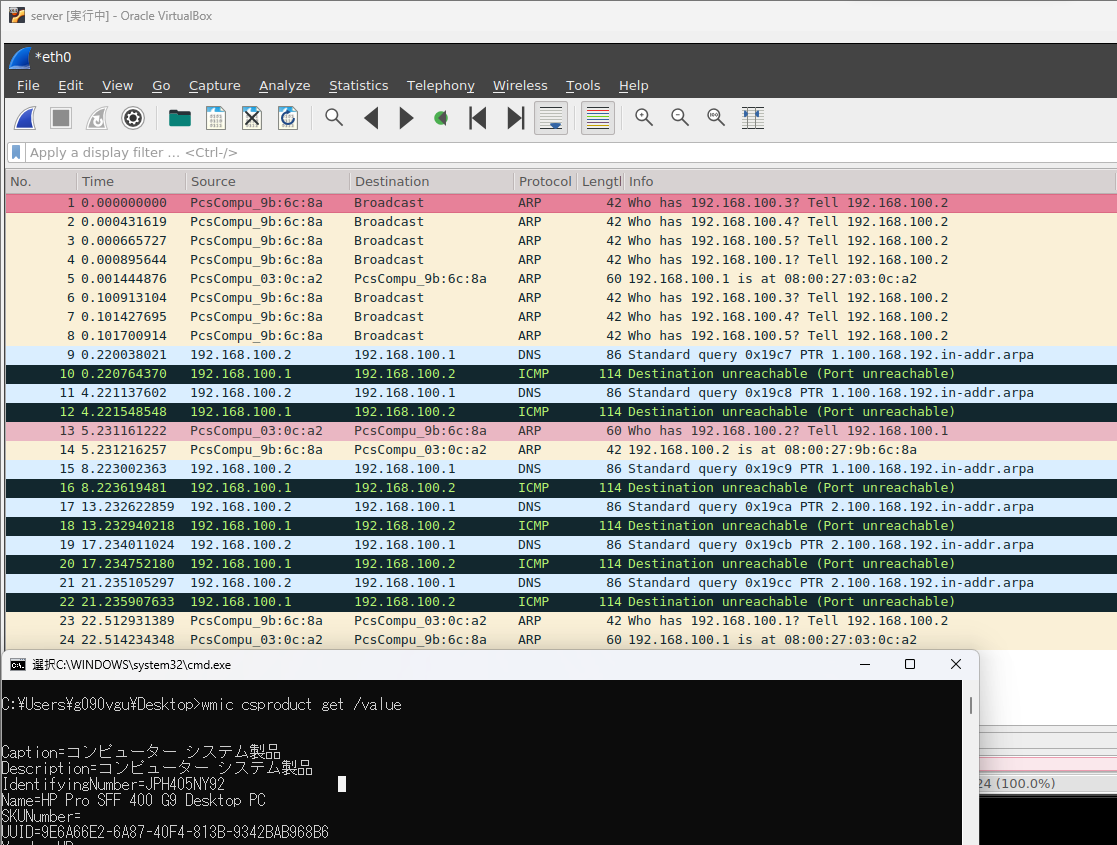
\includegraphics[width=0.8\textwidth]{imgs/1/nmap_ping_scan_result.png} 
            \caption{pingスキャン時にキャプチャされたパケット一覧}
            \label{fig:nmap_ping_scan_result}
        \end{figure}

        \begin{figure}[htbp]
            \centering
            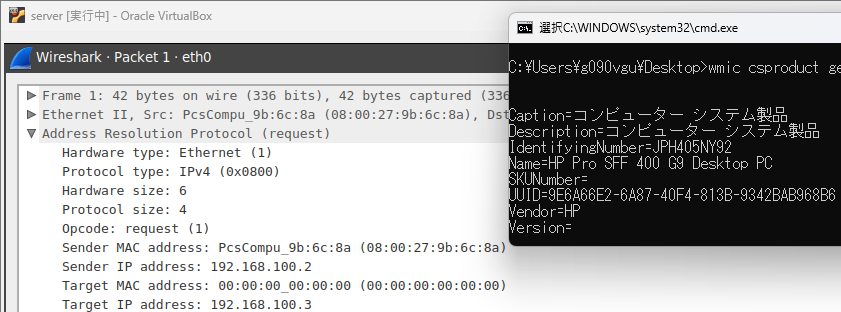
\includegraphics[width=0.8\textwidth]{imgs/1/nmap_ping_scan_result_arp_request.png} 
            \caption{ARPリクエスト}
            \label{fig:nmap_ping_scan_result_arp_request}
        \end{figure}

        \begin{figure}[htbp]
            \centering
            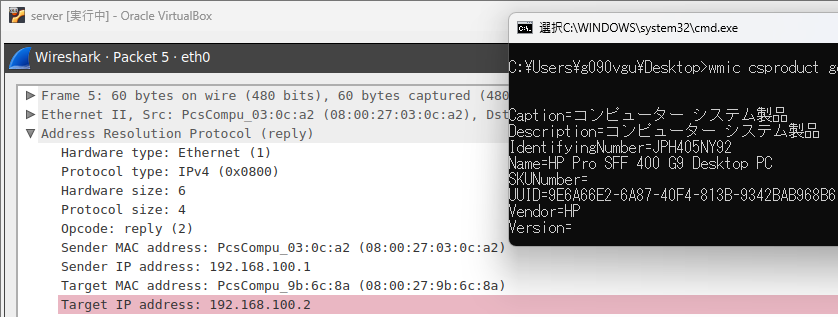
\includegraphics[width=0.8\textwidth]{imgs/1/nmap_ping_scan_result_arp_reply.png} 
            \caption{ARP応答}
            \label{fig:nmap_ping_scan_result_arp_reply}
        \end{figure}

        \begin{figure}[htbp]
            \centering
            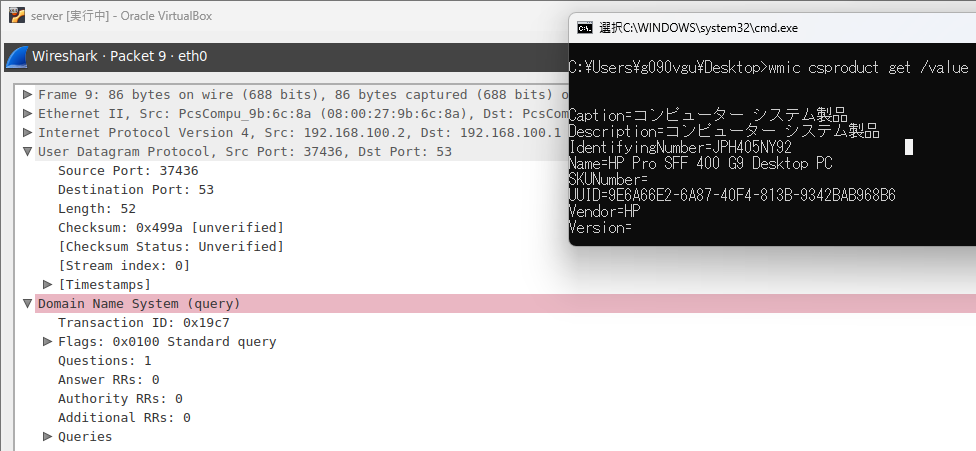
\includegraphics[width=0.8\textwidth]{imgs/1/nmap_ping_scan_result_dns.png} 
            \caption{DNS問い合わせ}
            \label{fig:nmap_ping_scan_result_dns}
        \end{figure}

        \begin{figure}[htbp]
            \centering
            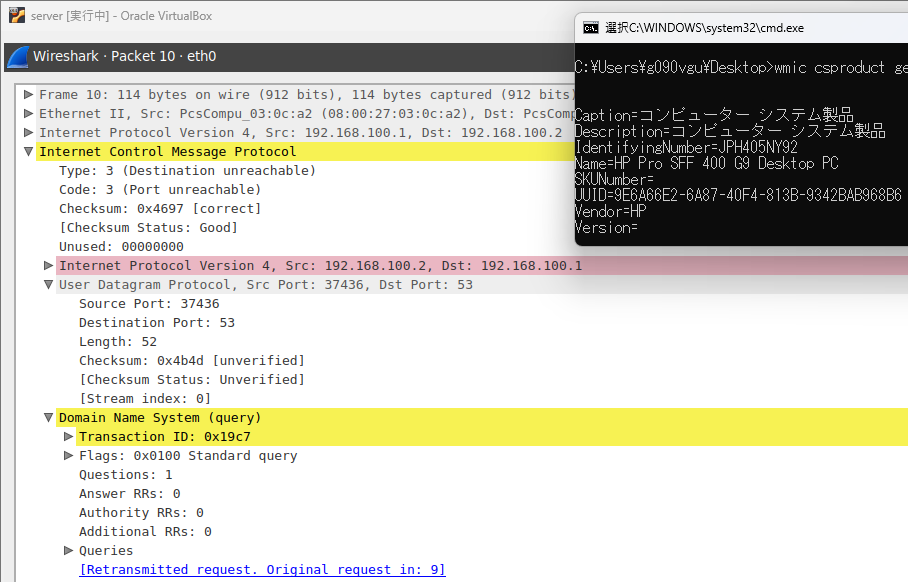
\includegraphics[width=0.8\textwidth]{imgs/1/nmap_ping_scan_result_icmp.png} 
            \caption{ICMP到達不能メッセージ}
            \label{fig:nmap_ping_scan_result_icmp}
        \end{figure}

    \end{enumerate}

    \vspace{0.5cm}
    \item Nmap を使ったポートスキャン \\
    サブゴール：探査用マシン(server)から，（１）ホスト検出で検出された各マシン（以下，被攻撃対象マシン）について順番に調査する
    \begin{enumerate}[label=\arabic*]
        \item telnet と ssh のポート番号以外の違いで最も大きな違いは何か調査しなさい．
        
        \quad
        telnetとsshはいずれもサーバ間のリモートアクセスに用いられるプロトコルであるが, sshでは通信内容が暗号化される一方でtelnetにおいては暗号化する仕組みがない\cite{telnet_ssh}.
        
        \item 3 種類のポートスキャンで，OSI 参照モデルのどの層で，どのような手順で，どのように，どのような情報が，やり取りされるか再確認し，整理しなさい．
        \item ［被攻撃対象マシン］で telnetd と dropbear と ftp が起動していないことを確認する．起動している場合には停止させる．起動しているかどうかは ps コマンドなどで確認すること． \\
        ※ ftp は ftp という文字を含むプログラムが動いていないことを確認
        \item ［探査用マシン］で Wireshark を起動し，以下の 4 つのポートスキャンによって生じた双方向の通信の内容を解析しなさい． \\
        ※ 先に以降の手順の意図を把握し，どのような結果を得るべきか考えて，解析をすることを奨める．また，適宜，解析を区切るなど，工夫して実施してもよい． \\
        ※ 結果の見通しをよくするためスキャン範囲を telnetd と dropbear が使用するポート番号の前後に絞ってもよいが、関係ないポートも一部含めること
        \begin{enumerate}[label=・]
            \item TCP connect スキャンを行う．
            \item SYN ステルススキャンを行う．
            \item UDP スキャンを行う．
            \item TCP/IP fingerprinting を用いて OS を判別する．
        \end{enumerate}
        \item ［被攻撃対象マシン］で telnetd と dropbear と ftp を起動させる．dropbear を起動させる際には，オプションとして -R をつけること．FTP server は，既にインストールされているソフト(GUI)を起動させればよい．
        \item telnetd と dropbear と ftp が起動していることを確認する．
        \item ［探査用マシン］から［被攻撃対象マシン］へ telnet および ssh で作成した一般権限ユーザ名でログインできることを確認する．
        \item ［探査用マシン］から［被攻撃対象マシン］へ telnet および ssh でログインする過程で生じた通信の内容を解析し，調査結果より想定される telnet と ssh の最も大きな違いが確認できることを，実験した結果（比較を含む）を用いて，レポートで報告しなさい． \\
        ヒント：TCP stream でログイン時のパケット内の情報について確認する
        \item 再び，手順 4.を実行し，以前の手順 4.での結果（出力とキャプチャパケットの面で）と比較し，整理した各ポートスキャンの動作の仕組み（OSI 参照モデルのどの層で，どのような手順で，どのように，どのような情報が，やり取りされるか）を，実験した結果（比較を含む）を用いて，レポートで報告しなさい．
        \item 手順 8.の比較の内，TCP/IP fingerprinting を用いた OS 判別において，3 つのポートスキャン方法の内，どの方法が利用されているか，実験した結果（比較を含む）を用いて，レポートで報告しなさい．また，OS の検出結果について違いが起きたか報告しなさい．
    \end{enumerate}
\end{enumerate}

\newpage

% --- 参考文献リストの出力 ---
\printbibliography[title=参考文献]

\end{document}